\documentclass[11pt, compress,xcolor=dvipsnames]{beamer}
\usepackage{booktabs}
\usepackage{color}
\usepackage{latexsym}
\usepackage{amsfonts}
\usepackage{amsmath}
\usepackage{multirow}
\usepackage[english]{babel}
\usepackage[utf8]{inputenc}
\usepackage{fancyhdr}
\usepackage{graphicx}
\usepackage{textcomp}
\usepackage{siunitx}
%\usepackage{bookmark}
%\usepackage{xcolor}
\usepackage{adjustbox}
% \usepackage{MnSymbol}

\usepackage{rotating}

%\usepackage{pstricks}
%\usepackage{pst-plot}

\usepackage{tikz}
\usepackage{tikzsymbols}
\usetikzlibrary{positioning,arrows,arrows.meta}
\usetikzlibrary{shapes.misc}
\tikzset{cross/.style={cross out, draw=black, minimum size=2*(#1-\pgflinewidth), inner sep=0pt, outer sep=0pt},
%default radius will be 1pt. 
cross/.default={1pt}} 
 

\definecolor{grigio}{gray}{0.25}
\newenvironment{sistema}%
{\left\lbrace\begin{array}{@{}l@{}}}%
{\end{array}\right.}
%\newcommand{\T}{$\mathbf{T}$}
%\DeclareMathOperator{\Tr}{Tr}
%\newcommand{\R}{\mathbb{R}}
\newcommand{\Rn}{\mathbb{R}^n}
\newcommand{\Rnn}{\mathbb{R}^{n\times n}}
%\usetheme{Frankfurt}
\usetheme{CambridgeUS}
\usecolortheme{beaver}
\useinnertheme{rounded}
\useoutertheme{miniframes}


%\setbeamercovered{invisible}
%\setbeamercovered{transparent}

\definecolor{rouge}{rgb}{0.9,0.1,0.2} 
\definecolor{bleu}{rgb}{0.4,0.2,0.9} 
\definecolor{vert}{rgb}{0.1,0.9,0.2} 
\definecolor{violet}{rgb}{0.9,0.1,0.8} 
\definecolor{rose}{rgb}{0.4,0.1,0.1} 
\DeclareMathOperator{\rank}{rank}

\def\bleu#1{{\color{blue}#1}}

%\newcommand{\bbm}{\begin{bmatrix}}
%\newcommand{\ebm}{\end{bmatrix}}
%\newcommand{\ip}[2]{\langle #1, #2 \rangle}
%\newcommand{\set}[1]{\left\{ #1 \right\}}
%\newcommand{\sbr}[1]{\left[ #1 \right]}
%\newcommand{\rbr}[1]{\left( #1 \right)}
%\newcommand{\norm}[1]{\left\| #1 \right\|}




%\usepackage[accumulated]{beamerseminar}

%\setbeamercovered{dynamic}
%\newcommand{\Lang}[1]{\operatorname{\text{\textsc{#1}}}}
%\newcommand{\Class}[1]{\operatorname{\mathchoice
%  {\text{\sf \small #1}}
%  {\text{\sf \small #1}}
%  {\text{\sf #1}}
%  {\text{\sf #1}}}}

\newcommand{\NumSAT}      {\text{\small\#SAT}}
\newcommand{\NumA}        {\#_{\!A}}
\newcommand{\barA}        {\,\bar{\!A}}
\newcommand{\Nat}{\mathbb{N}}
\newcommand{\Set}[1]{\{#1\}}
\newcommand{\bm}[1]{\mbox{\boldmath $ #1 $ }}
\newcommand{\model}[1]{\mbox{\boldmath$#1$\unboldmath}}
\newcommand{\emmodel}[1]{\mbox{\em {\bf #1}}}

\newcommand{\N}{\mathbb N}
\newcommand{\Z}{\mathbb Z}
\newcommand{\Q}{\mathbb Q}
\newcommand{\R}{\mathbb R}
\newcommand{\C}{\mathbb C}

\newcommand{\tq}{\; | \;}
\newcommand{\pv}{\; ; \;}

\newcommand{\DD}{\texttt{DD}}          %%%%%% 
\newcommand{\CD}{\texttt{CD}}          %%%%%% 

\def\lp{[}
\def\rp{]}

\newcommand{\hs}{\hspace*{1.0cm}}
\newcommand{\hst}{\hspace*{0.5cm}}
\newcommand{\hsh}{\hspace*{0.2cm}}
\newcommand{\vs}{\vspace*{0.5cm}}
\newcommand{\pp}{\vspace*{6 mm}}

\newcommand{\ov}{\overline}
\newcommand{\wh}{\widehat}
\newcommand{\ud}{\underline}

\newcommand{\ds}{\displaystyle}

\def \union{\mathop{\mathrm{\cup}}}

\def \equi{\Longleftrightarrow}
\newcommand{\ra}{\rightarrow}
\newcommand{\la}{\leftarrow}
\newcommand{\lara}{\leftrightarrow}
\newcommand{\Ra}{\Rightarrow}
\newcommand{\La}{\Leftarrow}
\newcommand{\longra}{\longrightarrow}
\newcommand{\longla}{\longleftarrow}
\newcommand{\Longra}{\Longrightarrow}
\newcommand{\Longla}{\Longleftarrow}
\newcommand{\benum}{\begin{enumerate}}
\newcommand{\eenum}{\end{enumerate}}
\newcommand{\bitem}{\begin{itemize}}
\newcommand{\eitem}{\end{itemize}}
\newcommand{\itemb}{\item[$\bullet$]}
\newcommand{\items}{\item[$\star$]}
\newcommand{\barray}{\begin{array}}
\newcommand{\earray}{\end{array}}
\newcommand{\btabular}{\begin{tabular}}
\newcommand{\etabular}{\end{tabular}}
\newcommand{\bfig}{\begin{figure}}
\newcommand{\efig}{\end{figure}}

\newtheorem{Def}{Definition}
\newtheorem{Th}{Theorem}
\newtheorem{Lem}{Lemma}
\newtheorem{Algo}{Algorithm}
\newtheorem{Propr}{Property}
\newtheorem{Propo}{Proposition}
\newtheorem{Cor}{Corollary}
\newtheorem{Rq}{Remark}
\newtheorem{Ex}{Example}
\newtheorem{Obs}{Observation}

\renewcommand{\theDef}{\thesection.\arabic{Def}}
\renewcommand{\theTh}{\thesection.\arabic{Th}}
\renewcommand{\theLem}{\thesection.\arabic{Lem}}
\renewcommand{\theAlgo}{\thesection.\arabic{Algo}}
\renewcommand{\thePropr}{\thesection.\arabic{Propr}}
\renewcommand{\thePropo}{\thesection.\arabic{Propo}}
\renewcommand{\theCor}{\thesection.\arabic{Cor}}
\renewcommand{\theRq}{\thesection.\arabic{Rq}}
\renewcommand{\theEx}{\thesection.\arabic{Ex}}
\renewcommand{\thefigure}{\thesection.\arabic{figure}}

\newcommand{\bEq}{\begin{equation}}
\newcommand{\eEq}{\end{equation}}
\newcommand{\bDef}{\begin{Def}}
\newcommand{\eDef}{\end{Def}}
\newcommand{\bTh}{\begin{Th}}
\newcommand{\eTh}{\end{Th}}
\newcommand{\bLem}{\begin{Lem}}
\newcommand{\eLem}{\end{Lem}}
\newcommand{\bAlgo}{\begin{Algo}}
\newcommand{\eAlgo}{\end{Algo}}
\newcommand{\bPropr}{\begin{Propr}}
\newcommand{\ePropr}{\end{Propr}}
\newcommand{\bPropo}{\begin{Propo}}
\newcommand{\ePropo}{\end{Propo}}
\newcommand{\bCor}{\begin{Cor}}
\newcommand{\eCor}{\end{Cor}}
\newcommand{\bRq}{\begin{Rq}}
\newcommand{\eRq}{\end{Rq}}
\newcommand{\bEx}{\begin{Ex}}
\newcommand{\eEx}{\end{Ex}}
\newcommand{\bFig}{\begin{figure}}
\newcommand{\eFig}{\end{figure}}
\newcommand{\Illustration}{\subsection*{Illustration:}}
\newcommand{\prf}{\noindent{\bf Proof:} }
\newcommand{\eprf}{$\blacksquare$}
\newcommand{\mqcr}{M}               %%%%%% 
\newcommand{\kqkp}{kQKP}               %%%%%% 
\newcommand{\imp}[1]{\textcolor{red}{#1}}
%\newcommand{\Rn}{\mathbb{R}^n}
\DeclareMathOperator{\Tr}{Tr}


\newcommand{\conv}{\text{conv}}

\newenvironment<>{problock}[1]{%
  \begin{actionenv}#2%
      \def\insertblocktitle{#1}%
      \par%
      \mode<presentation>{%
        \setbeamercolor{block title}{fg=white,bg=orange!20!black}
       \setbeamercolor{block body}{fg=black,bg=yellow!50}
       \setbeamercolor{itemize item}{fg=orange!20!black}
       }%
      \usebeamertemplate{block begin}}
    {\par\usebeamertemplate{block end}\end{actionenv}}


\newcommand{\executeiffilenewer}[3]{%
\ifnum\pdfstrcmp{\pdffilemoddate{#1}}%
{\pdffilemoddate{#2}}>0%
{\immediate\write18{#3}}\fi%
}
\newcommand{\includesvg}[1]{%
\executeiffilenewer{#1.svg}{#1.pdf}%
{inkscape -z -D --file=#1.svg  %
--export-pdf=#1.pdf --export-latex}%
\input{#1.pdf_tex}%
}

\title[Maximum Regrets 4 MDP]{Deterministic Solutions Based on Maximum Regrets in MDPs with Imprecise Rewards}
%\subtitle{\emph{S\'eminaire CNAM 2017}}
\author[P. Alizadeh]{Gugulino}
\institute[LIPN]{\emph{LIPN - CNRS - Univ. Paris 13 - USPC}}

\date[02/03/2018]{\normalsize{EGC 2019}\\Metz 21-25 Janvier 2019}

\begin{document}

\begin{frame}[plain]
\titlepage
\end{frame}


\section[Basic definitions]{Basic definitions and motivation}

\begin{frame}
\frametitle{MDP - basic definitions}

TODO

\end{frame}


\begin{frame}
\frametitle{Why MDPs?}
\imp{Markov Decision Processes (MDPs)} are effective models for representing and solving \imp{sequential decision problems}(autonomous vehicles, robotics or service composition).

\begin{itemize}
\item Applications: autonomous vehicles, robotics, service composition, $\dots$. 
\item Goal: maximize the expected sum of rewards.
\end{itemize}

\end{frame}


\begin{frame}
\frametitle{Why MDPs with Imprecise Rewards?}
It is \imp{often impossible to give an exact estimation of the data} describing a problem:
\begin{columns}
\begin{column}{0.69\textwidth}
\begin{itemize}
\item 
(1) \imp{insufficient data} to estimate the rewards,
\item 
(2) parts of models are \imp{too complex} to detail, % In assistant vehicle example, defining exact rewards for all actions is time consuming or complicated and can variate during the driving process. %For this reason, we consider them bounded in real valued intervals,
%\item 
\item 
(3) \imp{conflicting elicitations} from users. %In the assistant vehicle case, if the model is designed for different drivers with various preferences, even after a limited number of communications with drivers and diminishing the rewards imprecision to a smaller sets, the MDP is not precise yet. 
\end{itemize}
\end{column}
\begin{column}{0.28\textwidth}
\begin{figure}
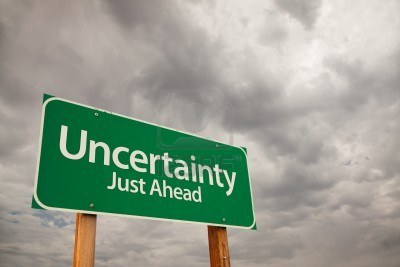
\includegraphics[height=0.25\textheight]{pics/uncertainty_data.jpg}
\end{figure}
\end{column}
\end{columns}
\pause
\begin{itemize}
\item We propose to find the policy that \imp{minimizes the maximum regret}.\\
\item Basic idea: to \imp{find the policy with the minimum lost} in \imp{comparison with
other possible policies} and reward instantiations.
\end{itemize}
\end{frame}


\begin{frame}
\frametitle{Min max regret- basic definitions}

TODO

\end{frame}


\begin{frame}
\frametitle{Stochastic vs deterministic policies}
\begin{itemize}
\item The majority of the exact and approximate methods for solving
an MDP accept to have \imp{stochastic policies}.\\
for a given state, the \textit{action} to be taken is chosen with a given \textit{probability} associated to each possible \textit{state}.
\item In a \imp{deterministic policy}, the \textit{action} to be taken in a state is \textit{uniquely defined}
\end{itemize}
\end{frame}

\begin{frame}
\frametitle{Stochastic vs deterministic policies}
\begin{itemize}
\item \textbf{Advantages} of stochastic policies:
\begin{itemize}
\item Finding an optimal stochastic policy is usually \imp{easier (faster) }than finding the optimal
deterministic policy.
\item Allowing stochastic policy = usually policies with a \imp{better value}.
\end{itemize}
\pause
\item \textbf{Disadvantages} of stochastic policies:
\begin{itemize}
\item A deterministic policy is \imp{easier to understand }from a user’s point of view.
\item A stochastic policy \imp{optimal only in expectation }on random
draws of actions.\\
$\Rightarrow$ It offers \textit{no guarantee of optimality if it is used only once} or for a short number of repetitions.
\end{itemize}
\end{itemize}
\end{frame}


\begin{frame}
\frametitle{Solution method}
\end{frame}


\begin{frame}
\frametitle{Solution method}
\end{frame}

\end{document}
